% =====================================================================
%  ch02e ------ 第 2 章 §2.5 + 小结 + 章末评注   译者：tr08
%  原书 p.93--p.99（PDF 113--119）
%  边界说明：p.93 顶部承接 ch02d 末尾的跨块句（$f$ 的作用式与「で表す」），
%            本块自「このことから，」起译；图 2.26 虽服务于 p.92 的讨论，
%            按 BRIEF §5 归本块。
% =====================================================================

% [原文 p.93]

\begin{figure}[htbp]
  \centering
  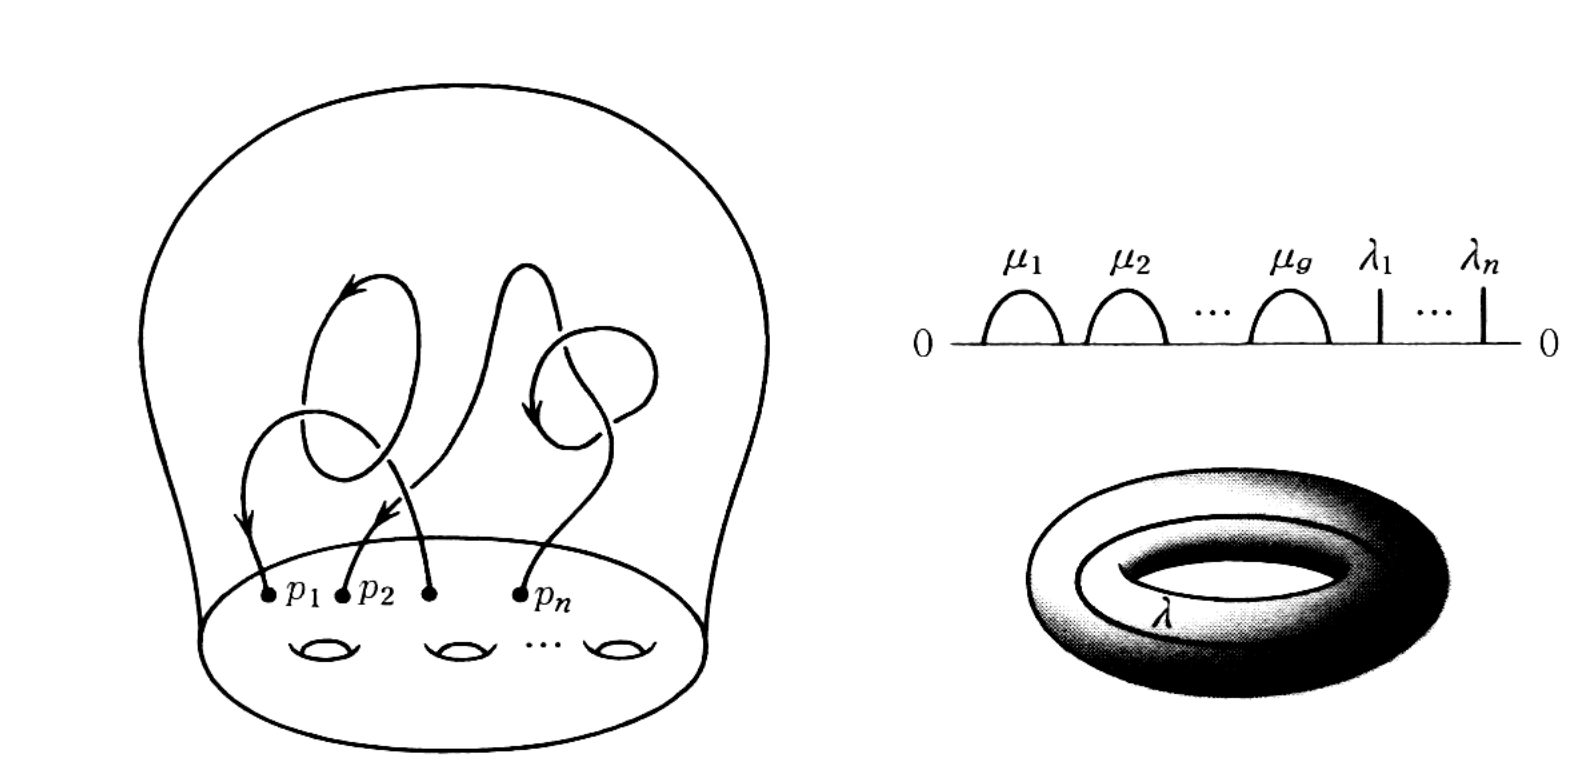
\includegraphics[width=0.92\textwidth]{figures/fig2.26.png}
  \figtitle{2.26}{原书无图注（原书 p.93）}
\end{figure}

由此，以 $C$ 的幂为模，
\begin{equation*}
  Z(M)=\sum_{\lambda}f_{0\lambda}\bigl\langle Z(M_{-}),\,v_{\lambda_1}\otimes\cdots\otimes v_{\lambda_m}\bigr\rangle
\end{equation*}
成立。这里 $\bigl\langle Z(M_{-}),\,v_{\lambda_1}\otimes\cdots\otimes v_{\lambda_m}\bigr\rangle$ 由式 (2.30) 就是赋予 framing $0$ 的链环 $L$ 的不变量 $S_{00}J(L;\lambda)$。再用式 (2.28) 所述的 $SL_2(\Z)$ 作用，就能在略去按 $C$ 的幂所作正规化的意义下，再现 $Z_k(M)$ 右端的形式。2.3 节中 $Z_k(M)$ 的定义稍显突兀，但这样看来便知：它可由 $SL_2(\Z)$ 在环面共形块空间上的作用自然描述。

% [Tutor Note: 此处的 $C$ 是前文 $Z_k(M)$ 归一化中出现的同一个符号，并非复数域 $\C$；“以 $C$ 的幂为模”意为结果只在相差 $C^{n}$ 的意义下相等。]
% [Tutor Note: $S_{00}J(L;\lambda)$ 是 $S$ 矩阵的 $(0,0)$ 元与 Jones 不变量之积；framing $0$ 指取零标架，改换标架会改变该值，故不可省略。]

\section{Chern--Simons 理论与曲面上联络空间的几何}

\takeaway{以 $SU(2)$ 主丛的联络空间 $\cA_M$ 为舞台：Chern--Simons 泛函的临界点恰为平坦联络，它在规范变换下只改变整数值；当 $\partial M=\Sigma$ 时，该泛函给出 $\cA_\Sigma$ 上的辛形式与复线丛 $L_\Sigma$ 及其联络，$Z_k(M)$ 则是共形块空间中的截面。}

设 $M$ 是定向三维流形。取 $G$ 为 Lie 群 $SU(2)$，$P$ 为 $M$ 上的 $SU(2)$ 主丛。$SU(2)$ 单连通，因此 $P$ 在拓扑上就是 $M$ 上的平凡 $SU(2)$ 丛。记 $P$ 的全体联络构成的空间为 $\cA_M$。$\cA_M$ 是仿射空间；取平凡联络为基点，把它与 $\Omega^{1}(M,\fg)$ 等同，后者由取值于 $G$ 的 Lie 代数 $\fg$ 的 $M$ 上一次微分形式构成。

% [原文 p.94]

该主丛 $P$ 的规范群（gauge group）$\cG$ 可看作从 $M$ 到 $G$ 的光滑映射全体构成的空间 $\Map(M,G)$。规范群 $\cG$ 通过拉回从右侧作用在联络空间 $\cA_M$ 上。具体地，这一作用由
\begin{equation}
  g^{*}A=g^{-1}Ag+g^{-1}\rd g,\qquad A\in\cA_M,\quad g\in\cG \tag{2.31}
\end{equation}
给出。此外，联络 $A$ 的曲率定义为
\begin{equation}
  F_A=\rd A+A\wedge A\in\Omega^{2}(M,\fg). \tag{2.32}
\end{equation}
对 $P$ 的联络 $A\in\cA_M$，令
\begin{equation}
  CS(A)=\frac{1}{8\pi^{2}}\int_{M}\Tr\Bigl(A\wedge \rd A+\frac{2}{3}A\wedge A\wedge A\Bigr),\qquad A\in\cA_M, \tag{2.33}
\end{equation}
并称 $CS$ 为 Chern--Simons 泛函（Chern--Simons functional）。

以下设 $M$ 的边界为空集，叙述 Chern--Simons 泛函的几条几何意义。

\begin{proposition*}{2.21}
  Chern--Simons 泛函 $CS\colon\cA_M\to\R$ 的临界点是平坦联络。
\end{proposition*}

\begin{proof}
  对联络的单参数族 $A_t=A+ta$，$CS(A+ta)$ 可用 $A$ 的曲率 $F_A=\rd A+A\wedge A$ 表为
  \begin{equation*}
    CS(A+ta)=CS(A)+\frac{t}{4\pi^{2}}\int_{M}\Tr(F_A\wedge a)+O(t^{2})
  \end{equation*}
  的形式。由此可知，$CS$ 的临界点是满足 $F_A=0$ 的联络 $A$，即平坦联络。
\end{proof}

用
\begin{equation*}
  B(\alpha,\beta)=\int_{M}\Tr(\alpha\wedge\beta)
\end{equation*}
定义双线性形式 $B\colon\Omega^{1}(M,\fg)\times\Omega^{2}(M,\fg)\to\R$，它非退化；借助 $B$，把 $\Omega^{2}(M,\fg)$ 看作 $\Omega^{1}(M,\fg)$ 的对偶空间。对联络 $A$，把给出其曲率 $F_A$ 的对应记为 $F$，则由 $\Omega^{2}(M,\fg)\cong\Omega^{1}(M,\fg)^{*}$，$F$ 可看作 $\cA_M$ 上的一次微分形式。

% [原文 p.95]

由
\begin{equation}
  \rd CS(A)=\frac{1}{4\pi^{2}}F_A \tag{2.34}
\end{equation}
可知 $F$ 是恰当形式。

% [Tutor Note: 式 (2.34) 中的 $\rd$ 是无限维空间 $\cA_M$ 上的微分（变分），不是 $M$ 上的外微分；系数 $1/4\pi^{2}$ 与 (2.33) 的 $1/8\pi^{2}$ 差因子 2，来自 $\delta(A\wedge\rd A)$ 两项的合并，可与命题 2.21 的展开式对照核对。]

接着叙述规范群对 Chern--Simons 泛函的作用。这里为了后面的讨论，也一并考察 $\partial M\neq\emptyset$ 的情形。

\begin{proposition}{2.22}
  \begin{equation}
    CS(g^{*}A)=CS(A)+\frac{1}{8\pi^{2}}\int_{\partial M}\Tr(A\wedge \rd g\,g^{-1})-\int_{M}g^{*}\sigma \tag{2.35}
  \end{equation}
  成立。这里 $\sigma$ 是由 (1.8) 给出的 $SU(2)$ 的体积元素。
\end{proposition}

特别地，$M$ 的边界为空集时，
\begin{equation}
  CS(g^{*}A)=CS(A)-\int_{M}g^{*}\sigma \tag{2.36}
\end{equation}
成立。右端出现的积分 $\int_{M}g^{*}\sigma$ 是 $g\colon M\to G$ 的映射度，恒为整数。因此，Chern--Simons 泛函诱导出从联络空间对规范群的商空间出发的映射
\begin{equation*}
  CS\colon\cA_M/\cG\longrightarrow\R/\Z.
\end{equation*}

% [Tutor Note: (2.36) 说明规范变换只把 $CS$ 改变一个整数值，这正是 $e^{2\pi\sqrt{-1}k\,CS}$ 在整数 $k$ 下规范不变的根源，也说明 $Z_k(M)$ 为何只对整数 $k$ 有定义。]

当 $\partial M\neq\emptyset$ 时，令 $\partial M=\Sigma$。记曲面 $\Sigma$ 上的 $G$ 主丛为 $Q$。这里同样取 $G=SU(2)$，所以拓扑上 $Q$ 同构于平凡丛 $\Sigma\times SU(2)$。记 $Q$ 的全体联络空间为 $\cA_\Sigma$；与三维流形的情形相同，$\cA_\Sigma$ 可与 $\Omega^{1}(\Sigma,\fg)$ 等同。又，对 $\alpha\in\cA_\Sigma$，切空间 $T_{\alpha}\cA_\Sigma$ 同构于 $\Omega^{1}(\Sigma,\fg)$。在切空间 $T_{\alpha}\cA_\Sigma$ 上，由
\begin{equation}
  \omega(\alpha,\beta)=-\frac{1}{8\pi^{2}}\int_{\Sigma}\Tr(\alpha\wedge\beta),\qquad \alpha,\beta\in\Omega^{1}(\Sigma,\fg) \tag{2.37}
\end{equation}
给出交错线性形式；它确定 $\cA_\Sigma$ 上的二次微分形式 $\omega$，非退化且满足 $\rd\omega=0$。由此，$\cA_\Sigma$ 具有无限维辛流形的结构。记 $Q$ 的规范群为 $\cG_\Sigma$。它可以看作光滑映射空间 $\Map(\Sigma,G)$。

% [原文 p.96]

以下叙述 $\cA_\Sigma$ 的几何与三维流形的 Chern--Simons 泛函之间的关系。

对 $\cA_\Sigma$ 的元素 $a$ 与规范群 $\cG_\Sigma$ 的元素 $g$，把联络 $a$ 到 $M$ 的扩张记为 $A$，把 $g$ 作为光滑映射到 $M$ 的扩张记为 $\tilde{g}\colon M\to G$，令
\begin{equation}
  c(a,g)=\exp\bigl(2\pi\sqrt{-1}\,(CS(\tilde{g}^{*}A)-CS(A))\bigr). \tag{2.38}
\end{equation}
具体地，它表为
\begin{equation}
  c(a,g)=\exp\Bigl(2\pi\sqrt{-1}\Bigl(\int_{\Sigma}\frac{1}{8\pi^{2}}\Tr(g^{-1}ag\wedge g^{-1}\rd g)-\int_{M}\tilde{g}^{*}\sigma\Bigr)\Bigr). \tag{2.39}
\end{equation}
第 2 项是 1.3 节所处理的 Wess--Zumino--Witten 模型中的 Wess--Zumino 项；右端不依赖 $g$ 的扩张 $\tilde{g}$ 的取法。因此，从积分的形式可知，右端只由 $\Sigma$ 上的 $a,g$ 决定。换个角度看，就等于证明了下面的命题。

\begin{proposition}{2.23}
  对以 $\Sigma$ 为边界的三维流形 $M$ 上的 Chern--Simons 泛函，关于规范群 $\Map(M,G)$ 的作用，利用 $M$ 上联络 $A$ 到 $\Sigma$ 的限制 $a$ 与 $g\in\Map(M,G)$ 到 $\Sigma$ 的限制 $g|_{\Sigma}$，
  \begin{equation}
    \exp\bigl(2\pi\sqrt{-1}\,CS(g^{*}A)\bigr)=c(a,g|_{\Sigma})\exp\bigl(2\pi\sqrt{-1}\,CS(A)\bigr) \tag{2.40}
  \end{equation}
  成立。
\end{proposition}

对 $\cA_\Sigma$ 的元素 $a$，记 $L_{\Sigma,a}$ 为满足
\begin{equation*}
  f(e\cdot g)=c(a,g)f(e),\qquad g\in\Map(\Sigma,G)
\end{equation*}
的映射 $f\colon\Map(\Sigma,G)\to\C$ 全体。$L_{\Sigma,a}$ 是带 Hermite 内积的一维复线性空间。由命题 2.23，当 $\partial M=\Sigma$ 时，对 $M$ 上的联络 $A$，令 $A$ 到 $\Sigma$ 的限制为 $a$，则 $\exp\bigl(2\pi\sqrt{-1}CS(A)\bigr)$ 自然地看作 $L_{\Sigma,a}$ 的元素。把 $\Sigma$ 的定向反转所得记为 $-\Sigma$，则
\begin{equation*}
  L_{-\Sigma,a}\cong\overline{L_{\Sigma,a}}
\end{equation*}
成立。设三维流形 $M$ 被曲面 $\Sigma$ 分成两部分，即 $M=M_1\cup M_2$，$\partial M_1=\Sigma$，$\partial M_2=-\Sigma$。把 $M$ 上的 $SU(2)$ 联络 $A$ 限制到 $M_1,M_2$ 上所得分别记为 $A_1,A_2$，再把 $A$ 到 $\Sigma$ 的限制记为 $\alpha$。此时
\begin{equation*}
  \exp\bigl(2\pi\sqrt{-1}\,CS_{M_1}(A_1)\bigr)\in L_{\Sigma,\alpha},\qquad
  \exp\bigl(2\pi\sqrt{-1}\,CS_{M_2}(A_2)\bigr)\in\overline{L_{\Sigma,\alpha}}
\end{equation*}
确定下来；利用自然配对 $L_{\Sigma,\alpha}\times L_{-\Sigma,\alpha}\to\C$，

% [Tutor Note: 原书定义 $L_{\Sigma,a}$ 时下标用一般元素 $a$，其后一律写作 $\alpha$（$\alpha$ 是 $A$ 到 $\Sigma$ 的限制）；两者是同一类对象，抄录时保留原样，勿据此后退修改公式。]

% [原文 p.97]

可以把 $\exp\bigl(2\pi\sqrt{-1}\,CS_M(A)\bigr)$ 表为
\begin{equation*}
  \Bigl(\exp\bigl(2\pi\sqrt{-1}\,CS_{M_1}(A_1)\bigr),\ \exp\bigl(2\pi\sqrt{-1}\,CS_{M_2}(A_2)\bigr)\Bigr).
\end{equation*}

又，把由 $\cA_\Sigma$ 的元素组成的单参数族 $\eta_t$（$0\le t\le 1$）看作 $\Sigma\times[0,1]$ 上的联络 $\eta$，则由以上的考察，通过 $\Sigma\times[0,1]$ 上的 Chern--Simons 泛函 $CS_{\Sigma\times[0,1]}$，给出映射
\begin{equation*}
  \exp\bigl(2\pi\sqrt{-1}\,CS_{\Sigma\times[0,1]}(\eta)\bigr)\colon L_{\Sigma,\eta_0}\longrightarrow L_{\Sigma,\eta_1}.
\end{equation*}
设 $L_\Sigma$ 是以 $L_{\Sigma,a}$ 为 $a$ 上纤维的 $\cA_\Sigma$ 上拓扑平凡的复线丛，则对联络空间 $\cA_\Sigma$ 的道路 $\eta_t$（$0\le t\le 1$），给出复线丛 $L_\Sigma$ 的提升。可以确定复线丛 $L_\Sigma$ 的联络，使这一提升成为水平截面。并且，作为该联络的曲率形式，$\cA_\Sigma$ 的辛形式得以再现。

如此，用 Chern--Simons 泛函，可以构造联络空间 $\cA_\Sigma$ 的道路到复线丛 $L_\Sigma$ 的提升；同样，用 Chern--Simons 泛函，也可以把规范群 $\cG_\Sigma$ 在 $\cA_\Sigma$ 上的作用提升到复线丛 $L_\Sigma$。对这一作用的矩映射 $\mu$，取 $\mu^{-1}(0)/\cG_\Sigma$，即 Marsden--Weinstein 商 $\cA_\Sigma/\!/\cG_\Sigma$，就得到 $\Sigma$ 上平坦 $G$ 联络的模空间 $\cM_\Sigma$ 及其上的复线丛 $\cL$。$\cM_\Sigma$ 可与 $\Sigma$ 的基本群 $\pi_1(\Sigma)$ 到 $G$ 的表示的等价类空间 $\Hom(\pi_1(\Sigma),G)/G$ 等同。

% [Tutor Note: 把 $\exp(2\pi\sqrt{-1}CS)$ 看成线丛的截面而非函数，是因为它依赖 $a$ 到 $M$ 的扩张 $A$；沿 $\cA_\Sigma$ 的道路走一圈（闭路）时按 $c(a,g)$ 作和乐平移，这正是“截面”而非“函数”的含义。]

设 $M$ 是紧致无边界定向三维流形，$k$ 为整数。Witten 给出的三维流形拓扑不变量形式上用路径积分表为
\begin{equation*}
  Z_k(M)=\int\exp\bigl(2\pi\sqrt{-1}\,k\,CS(A)\bigr)\,\mathcal{D}A.
\end{equation*}
对带边界的三维流形 $M$，把 $Z_k(M)$ 应取值的状态空间定式化，展开 2+1 维拓扑场论，这正是（本书的）目标。令 $\partial M=\Sigma$，$A$ 为 $M$ 上的 $G$ 联络，$\alpha$ 为 $A$ 到 $\Sigma$ 的限制。由以上的考察，

% [原文 p.98]

可以认为
\begin{equation*}
  \exp\bigl(2\pi\sqrt{-1}\,k\,CS(A)\bigr)\in L_{\Sigma,\alpha}
\end{equation*}
成立。记限制到 $\Sigma$ 上恰为 $\alpha$ 的 $M$ 上 $G$ 联络全体为 $\cA_\alpha$，形式上令
\begin{equation*}
  Z_k(M)(\alpha)=\int_{\cA_\alpha}\exp\bigl(2\pi\sqrt{-1}\,k\,CS(A)\bigr)\,\mathcal{D}A,
\end{equation*}
则由
\begin{equation*}
  \exp\bigl(2\pi\sqrt{-1}\,k\,CS(g^{*}A)\bigr)=c(g,\alpha)^{k}\exp\bigl(2\pi\sqrt{-1}\,k\,CS(A)\bigr)
\end{equation*}
可知，$Z_k(M)$ 确定复线丛 $\cL^{\otimes k}$ 的截面。

% [Tutor Note: 原书 p.98 此处印作 $c(g,\alpha)$，与 (2.38) 中 $c(a,g)$ 的自变量次序相反；按定义（$a$ 取在 $\cA_\Sigma$，$g$ 取在规范群）应为 $c(\alpha,g)$。疑为笔误，正文照录原文。]

上面的平坦联络模空间 $\cM_\Sigma$ 可以如下引入复结构。如 Atiyah--Bott [15] 所示，$\cM_\Sigma$ 可与 $\Sigma$ 上拓扑平凡的全纯 $G_\C$ 丛的模空间等同，从而带有由 $\Sigma$ 的复结构 $J$ 导出的复结构。把这样赋予复结构的 $\cM_\Sigma$ 记为 $\cM_\Sigma^{(J)}$。再引入 Kähler 极化，记 $\cM_\Sigma$ 上复线丛 $\cL^{\otimes k}$ 的全纯截面全体构成的空间为 $\cH_\Sigma$，并把它看作状态空间。$\cH_\Sigma$ 是有限维复线性空间，已知它与 $\Sigma$ 的共形块空间同构。请参看文献 [19] 等。这样就能看出 Chern--Simons 理论与共形场理论之间的联系。特别地，作为复线性空间，$\cH_\Sigma$ 与 2.4 节构成的 $Z_\Sigma$ 同构。

% [Tutor Note: Kähler 极化指在 $\cM_\Sigma$ 上取定与辛形式相容的复结构；不同的极化给出同一空间的不同模型（正则是“全纯截面”相对哪个复结构而言），作者未讨论其依赖，引用文献 [19] 处理。]

其次提一下三维流形含链环的情形。设 $M$ 是紧致闭定向三维流形，$M$ 含链环 $C_1\cup\cdots\cup C_r$。让 $C_j$ 对应 Lie 群 $G$ 的表示 $R_j$，令
\begin{equation*}
  W_{C_j,R_j}(A)=\Tr_{R_j}\mathrm{Hol}_{C_j}(A).
\end{equation*}
这里右端是把沿曲线 $C_j$ 的联络 $A$ 的和乐取表示 $R_j$ 的迹。此时，Witten 不变量由
\begin{equation}
  Z_k(M;C_1,\cdots,C_r)=\int\exp\bigl(2\pi\sqrt{-1}\,k\,CS(A)\bigr)\prod_{j=1}^{r}W_{C_j,R_j}(A)\,\mathcal{D}A \tag{2.41}
\end{equation}
给出。与上述路径积分相应的状态空间，由抛物向量丛的模空间理论定式化。

% [Tutor Note: (2.41) 中的路径积分是形式记号，$\mathcal{D}A$ 没有测度意义；本节所有含 $\int\mathcal{D}A$ 的等式都只在微扰展开（第 3 章）的意义下理解。]

% [原文 p.99]

\section*{小结}
\addcontentsline{toc}{section}{小结}
\markright{小结}

\takeaway{本章四条主线：KZ 单值给出辫群表示、共形块和乐给出 Jones 多项式的单位根特殊值、共形场论构造 Witten 不变量并验证 Atiyah 公理、Chern--Simons 泛函在曲面上联络空间上给出线丛与联络。}

\textbf{《要约》}

\textbf{2.1}\quad 研究了作为 KZ 方程的单值表示出现的辫群表示的结构，并证明在特殊情形下可得到经由 Iwahori--Hecke 代数的表示。

\textbf{2.2}\quad 利用共形块空间的和乐，证明了可以求得 Jones 多项式在 1 的单位根处的特殊值。

\textbf{2.3}\quad 从共形场理论的角度构造了三维流形的 Witten 不变量。进而证明了 Atiyah 意义下的拓扑场论的例子可以给出。

\textbf{2.4}\quad 证明了带边界的三维流形的 Chern--Simons 泛函确定曲面上联络空间上的复线丛及其联络。

% [Tutor Note: 原书《要約》只列 2.1--2.4 四条，没有 §2.5，这是原书面貌，不是漏译；§2.5 的内容（联络空间的辛几何与复线丛）可视为 2.3、2.4 的技术准备。]
% [Tutor Note: 2.1 条的“特殊情形”指 $G=SU(m)$、$V$ 取 $m$ 维自然表示：此时 KZ 表示经由 Iwahori--Hecke 代数分解；一般情形的单值群并不落在 Hecke 代数像中。]
% [Tutor Note: 2.2 条的“1 的单位根”即 $q=e^{2\pi\sqrt{-1}/k}$ 型单位根；此时 $U_q(\fsl_2)$ 的表示论给出 Jones 多项式的特殊值，这是量子群与共形场论相通的入口。]

\chapterreview{%
\textbf{（一）全章地位。}第 2 章是全书的技术枢纽。第 1 章搭起的共形场理论语言，在本章兑现为一个具体的三维拓扑不变量：KZ 方程的单值、共形块的和乐、环面上的 $SL_2(\Z)$ 作用与 Chern--Simons 路径积分被拼在一起，Witten 由物理的路径积分给出 Jones 多项式与三维流形不变量的统一解释，本章则把这一解释逐步改写成可检验的数学陈述。

\textbf{（二）知识脉络。}全章沿三条线索推进。其一，从 KZ 方程出发得到辫群的表示，在特殊情形下经过 Iwahori--Hecke 代数（§2.1）；其二，用共形块空间的和乐取出 Jones 多项式在单位根处的特殊值（§2.2）；其三，把共形块丛、映射类群的射影表示与配分函数组装成三维流形的 Witten 不变量，并验证 Atiyah 公理意义下的拓扑场论（§2.3、§2.4）。§2.5 再从 Chern--Simons 泛函出发重做一遍：临界点、辛形式、复线丛与平坦联络模空间上的全纯截面，逐层对应到前面的共形块。

\textbf{（三）核心结论。}可归纳为四点。Chern--Simons 泛函的临界点恰是平坦联络；它在规范变换下只改变整数值，故 $e^{2\pi\sqrt{-1}k\,CS}$ 在整数 $k$ 下规范不变。$\partial M=\Sigma$ 时，泛函给出 $\cA_\Sigma$ 上的辛形式 $\omega$、复线丛 $L_\Sigma$ 及曲率为 $\omega$ 的联络。$Z_k(M)$ 是该线丛 $k$ 次张量幂的截面，其截面空间与 $\Sigma$ 的共形块空间同构。带链环时插入和乐的迹，便得到 $Z_k(M;C_1,\dots,C_r)$。

\textbf{（四）辨析与提醒。}读本章要盯住三处约定。第一是符号 $C$ 与 $c(a,g)$：前者是 $Z_k(M)$ 归一化中的因子，后者是定义在 $\cA_\Sigma\times\cG_\Sigma$ 上的余循环；原书 p.98 印作 $c(g,\alpha)$，次序与 (2.38) 相反，应读作 $c(\alpha,g)$。第二是 $a$ 与 $\alpha$：$a$ 泛指 $\cA_\Sigma$ 的元素，$\alpha$ 专指 $A$ 到 $\Sigma$ 的限制，原书在两者间切换而未声明。第三是 $1/8\pi^{2}$、$1/4\pi^{2}$ 与 $2/3$ 的配合：它们由 $\rd CS=\frac{1}{4\pi^{2}}F_A$ 与 $\rd CS=\frac{1}{8\pi^{2}}\Tr(F\wedge F)$ 的相容性唯一确定，换一本书的归一化就会差 $2\pi$ 因子。

\textbf{（五）评注。}本章许多论证仍是“物理级别”的：路径积分没有测度，$Z_k(M)$ 的构造依赖文献 [19] 的共形块理论，$k\to\infty$ 的渐近展开也只是提示。真正的严格化要等第 3 章的微扰理论：把 $1/k$ 当作展开参数，用 Feynman 图与 Kontsevich 积分逐阶计算，才能把 Witten 不变量的各级系数落实为 Vassiliev 不变量。因此本章最好像读一份施工图：先接受整体框架，把每个等式的含义弄清，再带着“哪里还没证明”的问题进入第 3 章。}

% CHUNK ch02e DONE


